\chapter{Evaluation/Messungen}\vspace{1cm}
\label{chp:eval}
% colors
\definecolor{turquoise}{rgb}{0 0.41 0.41}
\definecolor{rouge}{rgb}{0.79 0.0 0.1}
\definecolor{vert}{rgb}{0.15 0.4 0.1}
\definecolor{mauve}{rgb}{0.6 0.4 0.8}
\definecolor{violet}{rgb}{0.58 0. 0.41}
\definecolor{orange}{rgb}{0.8 0.4 0.2}
\definecolor{bleu}{rgb}{0.39, 0.58, 0.93}



Im Kapitel Evalution/Messungen soll das in dieser Arbeit implementierte Programm analysiert und bewertet werden. Gemessen wurden das Einlesen und Schreiben der Daten, die dynamische Konfiguration der Fehlerwerte, sowie der Injektionsvorgang mit den verschiedenen Injektionsstrategien. Im Fokus der Messungen stand prim\"ar die Laufzeit der Fehlerinjektionen, ebenso wurden CPU-Auslastung und Speicherverbrauch untersucht. 

\section{Testaufbau} 
F\"ur die Messungen der Funktionen wurde der folgende Testaufbau umgesetzt: Softwareseitig wurde das System Ubuntu 12.04 mit der Kernel Version 3.2.0-26-generic-pae eingesetzt. Die verwendete Javassist Library ist in Version 3.12.0.GA in die Anwendung integriert worden. Auf der Hardwareseite wurde ein Intel Core i7-2630QM Prozessor mit 8 $\times$ 2.00GHz und einem Arbeitsspeicher von 7.8 GiB verwendet.\\
Die konkreten Messergebisse konnten mit Hilfe des Tools VisualVM Version 1.3.4\footnote{http://visualvm.java.net/relnotes.html - Zugriff 16.09.12} bestimmt werden. Das Tool zeichnet die Aktivit\"aten eines gew\"ahlten Prozesses auf und gibt diese als Diagramm im Reiter Monitor wieder. Alle Laufzeitmessungen wurden direkt im Java Code integriert. Als Testinput dient eine 51.2MB gro\ss e, durch den Output von /dev/zero\footnote{Unix virtuelle Gerätedatei, liefert Null-Bytes}, generierte Datei. Die getesteten Methoden wurden nicht separat sondern, wie in der Anwendung auch, \"uber das \courier{Controller}-Objekt aufgerufen. Die Messung der Strategien wurden jeweils f\"ur die Blockgr\"o\ss en 1, 8, 128, 1024 und 2048 mit den Fehlerraten 1\%, 5\%, 10\%, 50\% und 100\% durchgef\"uhrt.

\section{Lese- und Schreiboperatinen}

F\"ur die Analyse der Einleseoperation ist die Method \courier{loadStream} evaluiert worden. Die folgenden Messwerte aus Tabelle \ref{tblEinlesen} beziehen sich auf das Einlesen der 51.2 MB Datei und der Daten\"ubergabe an das \courier{Context} Objekt.\\
Die Laufzeitmessungen der Methode \courier{loadStream} ergaben einen Mittelwert von 2650 Millisekunden. Versuche mit anderen Java Streams konnten keine nennenswerten Verbesserungen erzielen. Die CPU-Auslastung der Methode stieg bei den Messungen durchschnittlich auf 20\% bis 25\% an. Der Speicherverbrauch lag bei den knapp unter 600 MB. Beim Schreiben der Daten durch die beiden unterschiedlichen Streams war der Laufzeitunterschied signifikanter. Die \courier{reduce} Methode wurde mit dem \courier{ObjectOutputStream} f\"ur serialisierbare Objekte und dem \courier{FileChannel} getestet. Die Umsetzung mit dem \courier{FileChannel} hat eine durchschnittliche Laufzeit von ca. 242 ms. Zum Schreiben der Daten als persistentes Objekt in Form der kompletten Java Liste bedarf es hingegen 113,88 Sekunden.\\

\begin{table}[!htbp]
\centering
\begin{tabular}{c|c|c|c|}
loadStream & Laufzeit & CPU-Last & Speicher\\
\hline
& 2650 ms & 20\% bis 25\% & $<$600 MB\\
\end{tabular}
\caption{Messwerte Einlesen und Daten\"ubergabe}
\label{tblEinlesen}
\end{table}

\section{Dynamische Konfiguration der Fehlerwerte}

Der folgende Test bezieht sich ausschlie\ss lich auf die Funktionalit\"at der dynamischen Fehlerregulierung bzw. der Manipulierung der Annotationen zur Laufzeit. F\"ur die Messungen wurden einem aktiven Stream der Klasse \courier{StreamProcessor} 50 \courier{FaultInj} Annotationen beigef\"ugt. Im Testlauf wurden alle 50 Annotationen mit neuen Werten belegt und die Klasse \courier{StreamProcessor} neu geladen.\\
Die Laufzeitmessung ergab einen Durschnittswert von 1.01 Sekunden. F\"ur den Normalfall einer einzelnen Fehlermodifikation liegt der Wert bei 220 ms. Demnach wird die meiste Zeit f\"ur den Reload des modifizierten \courier{StreamProcessor's} verwendet. Die CPU-Auslastung und der Speicherverbrauch sind in Abbildung \ref{tblDymFehler} grafisch dargestellt. Bei der CPU-Auslastung konnte ein kontinuierlicher Anstieg bis auf knapp 20\% ermittelt werden. Der Speicherverbrauch stieg w\"ahrend der Methodenausf\"uhrung von 10 auf 15 MB nur geringf\"ugig an. 

\begin{figure}[!htb]

\begin{minipage}{7.5cm}

%1950=0 4
\psset{xunit=0.1cm, yunit=0.1cm } 
\begin{pspicture}(-15 , -20)(50,60)
\psaxes[Dx=1, dx=50, Dy=10, dy=10, Ox=0]{->}(60,60) % x=70*0.1=7cm; Dx shown start value; dx*0.1 is distance 
\uput[-90](30,-8){\textcolor{blue}{Zeit in s}}
\uput[180]{90}(-10,30){\textcolor{blue}{CPU-Last in \%}}
\readdata{\data}{cpuAnno.dat} 
\listplot[showpoints=true,linecolor=red, linewidth=1.5pt]{\data}
\end{pspicture}

\end{minipage}
\begin{minipage}{7cm}

%1950=0 4
\psset{xunit=0.1cm, yunit=0.1cm } 
\begin{pspicture}(-20 ,-20)(50,60)
\psaxes[Dx=1, dx=50, Dy=10, dy=10, Ox=0]{->}(60,60) % x=70*0.1=7cm; Dx shown start value; dx*0.1 is distance 
\uput[-90](30,-8){\textcolor{blue}{Zeit in s}}
\uput[180]{90}(-10,30){\textcolor{blue}{Speicherverbrauch in MB}}
\readdata{\data}{memoryAnno.dat} 
\listplot[showpoints=true,linecolor=red, linewidth=1.5pt]{\data}
\end{pspicture}

\end{minipage}

\caption{Messung dynamische Fehlerregulierung}
\label{tblDymFehler}
\end{figure}


\section{Injektionsstategien}

\definecolor{myblue}{HTML}{92dcec}
\newcommand\VRule[1][\arrayrulewidth]{\vrule width #1}

\subsection*{Strategie Random}

Die Random Strategie hat von allen Block-Strategien die l\"angste Laufzeit. Dies resultiert aus der zus\"atzlichen Generierung von zuf\"alligen Bytes.\\
In Abbildung \ref{diaRandom} ist zu sehen wie die Laufzeit bei einer Blockvergr\"o\ss erung sehr stark abnimmt, im Vergleich zu den \"ubrigen Strategien. Je gr\"o\ss er der Block, um so seltener muss die Zufallsgenerierung aufgerufen werden. Sie kann in diesem Fall bereits die Bytes für den ganzen Block in einer Interation generieren. Bei einer Blockgr\"o\ss e von 1 ruft die Funktion f\"ur jedes zu injizierende Byte die Zufallsgenereriung erneut auf, was zu einem Anstieg der Laufzeit f\"uhrt. \\
Entsprechend verh\"alt es sich auch mit der Fehlerrate, wie die Werte aus Tabelle \ref{tblRandom} verdeutlichen. Bei einer steigenden Fehlerrate verl\"angert sich die Laufzeit, da mehr Bytes injiziert werden m\"ussen und entsprechend häufig eine Zufallsgenerierung verlangt wird. Dementsprechend m\"ussen bei einer Fehlerrate von 1.0 f\"ur jeden Block neue Zufallsbytes erstellt werden, was zu einem deutlichen Mehraufwand f\"uhrt. \\ 

\begin{table}[!htb]

\begin{tabular}{rrrrrrr}
\hline\\
\multicolumn{0}{c}{\colorbox{myblue}{\textbf{RANDOM}}} &  
\multicolumn{0}{c}{\colorbox{myblue}{\textbf{Block}}} &  
\multicolumn{0}{c}{\colorbox{myblue}{\textbf{Rate: 0.01}}} &  
\multicolumn{0}{c}{\colorbox{myblue}{\textbf{Rate: 0.05}}} & 
\multicolumn{0}{c}{\colorbox{myblue}{\textbf{Rate: 0.1}}} &
\multicolumn{0}{c}{\colorbox{myblue}{\textbf{Rate: 0.5}}} & 
\multicolumn{0}{c}{\colorbox{myblue}{\textbf{Rate: 1.0}}}\\
 & 1 & 2.84 s & 2.91 s & 3.00 s & 3.85 s & 4.37 s \\
 & 8 & 0.85 s & 0.86 s & 0.89 s & 1.33 s & 1.69 s \\
 & 128 & 0.58 s & 0.59 s & 0.65 s & 0.96 s & 1.30 s \\ 
 & 1024 & 0.54 s & 0.58 s & 0.62 s & 0.91 s & 1.28 s \\
 & 2048 & 0.53 s & 0.57 s & 0.61 s & 0.90 s & 1.26 s \\
\hline
\end{tabular}
\caption{Messwerte Random Strategie}
\label{tblRandom}
\end{table}
\begin{figure}[!htb]

\begin{tikzpicture}
	
	\drawlegend		
 
  \draw (0cm,0cm) -- (13.5cm,0cm);  %Abzisse
  \draw (0cm,0cm) -- (0cm,-0.1cm);  %linkes Ende der Abzisse
  \draw (13.5cm,0cm) -- (13.5cm,-0.1cm) node [right] {Rate}; %rechtes Ende der Abzisse
  
  \draw (-0.1cm,0cm) -- (-0.1cm,5.5cm);  %Ordinate
  \draw (-0.1cm,0cm) -- (-0.2cm,0cm);  %unteres Ende der Ordinate
  \draw (-0.1cm,5.5cm) -- (-0.2cm,5.5cm) node [left] {t in s};  %oberes Ende der Ordinate

  \foreach \x in {2,4,6,8,10}  %Hilfslinien
    \draw[gray!50, text=black] (-0.2 cm,0.5*\x cm) -- (13.5 cm,0.5*\x cm) 
      node at (-0.5 cm,0.5*\x cm) {\x};  %Beschriftung der Hilfslinien

 %   \node at (7.5cm,6cm) {Injektionsstrategie Random mit Lese- und Scheiboperationen};  	%Überschrift  
    
  \foreach \x/\y/\country in {%0.5/1.446/unmodified,  %\x ist Anfang der Säulen
                              0.5/2.84/Rate 0.01,  %\y ist Höhe der Säulen
                              3.0/2.91/Rate 0.05,
                             % 5/33.89/Rate 0.5,
                              5.5/3.00/Rate 0.1,
                             % 8/1.5/Niederlande,
                              8.0/3.85/Rate 0.5 ,
                             % 11/0.9/Deutschland,
                              10.5/4.37/Rate 1.0}%,
                             % 14/0.1/Italien}
    {
     \drawRecA{(\x cm,0cm) rectangle (0.4cm+\x cm, 1.446cm + 0.5*\y cm);}%die Säulen
     %  node at (0.5cm + \x cm,\y cm + 0.3cm) {\y}; %die Prozente über den Säulen
     %\node[rotate=45, left] at (0.6 cm +\x cm,-0.1cm) {{\tiny \country}}; %Säulenbeschriftung
    };      
          
  \foreach \x/\y/\country in {0.9/0.85/Rate 0.01,  %\x ist Anfang der Säulen
                              3.4/0.86/Rate 0.05,
                              5.9/0.89/Rate 0.1,
                              8.4/1.33/Rate 0.5,
                              10.9/1.69/Rate 1.0}
    {
     \drawRecB{(\x cm,0cm) rectangle (0.4cm+\x cm, 1.446cm + 0.5*\y cm);} %die Säulen
    };    

  \foreach \x/\y/\country in {1.3/0.58/Rate 0.01,  %\x ist Anfang der Säulen
                              3.8/0.59/Rate 0.05,
                              6.3/0.65/Rate 0.1,
                              8.8/0.96/Rate 0.5,
                              11.3/1.30/Rate 1.0}
    {
     \drawRecC{(\x cm,0cm) rectangle (0.4cm+\x cm, 1.446cm + 0.5*\y cm);} %die Säulen
     %  node at (0.5cm + \x cm,\y cm + 0.3cm) {\y}; %die Prozente über den Säulen
     \node[rotate=45, left] at (0.6 cm +\x cm,-0.1cm) {\country}; %Säulenbeschriftung
    }; 

  \foreach \x/\y/\country in {1.7/0.54/Rate 0.01,  %\x ist Anfang der Säulen
                              4.2/0.58/Rate 0.05,
                              6.7/0.62/Rate 0.1,
                              9.2/0.91/Rate 0.5,
                              11.7/1.28/Rate 1.0}
    {
     \drawRecD{(\x cm,0cm) rectangle (0.4cm+\x cm, 1.446cm + 0.5*\y cm);} %die Säulen
    }; 
    
  \foreach \x/\y/\country in {2.1/0.53/Rate 0.01,  %\x ist Anfang der Säulen
                              4.6/0.57/Rate 0.05,
                              7.1/0.61/Rate 0.1,
                              9.6/0.90/Rate 0.5,
                              12.1/1.26/Rate 1.0}
    {
    \drawRecE{(\x cm,0cm) rectangle (0.4cm+\x cm, 1.446cm + 0.5*\y cm);} %die Säulen
    };    
 
    	\draw[black, text=black, line width=1.5pt, style=dashed] (-0.5 cm,1.446 cm) -- (13.5 cm,1.446 cm); %Baseline     
	\node at (13.5cm,1.7cm) {Baseline\footnotemark};  %Überschrift    
      
    
\end{tikzpicture}

\caption[Messung Random Strategie]{Injektionsstrategie Random mit Lese- und Scheiboperationen}
\label{diaRandom}
\end{figure}


%====================================
\subsection*{Strategie Loss}
%===================================
Die Loss Strategie wurde anfangs durch eine einfache L\"oschoperation in der Liste realisiert. Diese Variante stellte sich allerdings als sehr ineffizient heraus, da die interne Umstruktierung durch das L\"oschen die Anwendung erheblich verlangsamt. Die Messung f\"ur die 51,2 MB Testdatei wurde nach etwas 5 Minuten abgebrochen. Eine 1 MB Datei konnte innerhalb von 61,2 Sekunden injiziert werden.  \footnotetext{Ausf\"uhrung ohne Fehlerinjektion}\\
Um das L\"oschen der Elemente zu umgehen wurde ein zweiter Ansatz gew\"ahlt, bei dem alle nicht injizierten Bytes einer neuen Liste angehangen werden. In der Auswertung aus Tabelle \ref{tblLoss} spiegelt sich diese Art der Implementierung wieder. Im Gegensatz zu allen anderen Strategien verlaufen die Balken im Diagramm aus Abbildung \ref{diaLoss} absteigend, je gr\"o\ss er die Fehlerrate gew\"ahlt wurde. Dies resultiert aus der Tatsache, dass die Methode die injizierten Bytes einfach ignoriert und nur alle nicht injizierten Bytes in die Liste aufnimmt. Eine Ausnahme bildet die Blockg\"o\ss e 1, bei der sich das \"uberspringen der injizierten Bytes erst ab einem Wert gr\"o\ss er als 0.5 lohnt. Eine detaillierte Begr\"undung dieses Ph\"anomens gibt es im Abschnitt \ref{BranchPrediction} \"uber Branch Prediction.\\

\begin{table}[!htb]

\begin{tabular}{rrrrrrr}
\hline\\
\multicolumn{0}{c}{\colorbox{myblue}{\textbf{LOSS}}} &  
\multicolumn{0}{c}{\colorbox{myblue}{\textbf{Block}}} &  
\multicolumn{0}{c}{\colorbox{myblue}{\textbf{Rate: 0.01}}} &  
\multicolumn{0}{c}{\colorbox{myblue}{\textbf{Rate: 0.05}}} & 
\multicolumn{0}{c}{\colorbox{myblue}{\textbf{Rate: 0.1}}} &
\multicolumn{0}{c}{\colorbox{myblue}{\textbf{Rate: 0.5}}} & 
\multicolumn{0}{c}{\colorbox{myblue}{\textbf{Rate: 1.0}}}\\
 & 1 & 3.44 s & 3.47 s & 3.56 s & 3.86 s & 2.79 s \\
 & 8 & 1.52 s & 1.47 s & 1.45 s & 1.27 s & 0.86 s \\
 & 128 & 1.17 s & 1.15 s & 1.13 s & 0.89 s & 0.60 s \\ 
 & 1024 & 1.16 s & 1.13 s & 1.12 s & 0.88 s & 0.57 s \\
 & 2048 & 1.14 s & 1.12 s & 1.11 s & 0.88 s & 0.57 s \\
\hline
\end{tabular}
\caption{Messwerte Loss Strategie}
\label{tblLoss}
\end{table}

\begin{figure}[!htb]

\begin{tikzpicture}

	\drawlegend 
 
  \draw (0cm,0cm) -- (13.5cm,0cm);  %Abzisse
  \draw (0cm,0cm) -- (0cm,-0.1cm);  %linkes Ende der Abzisse
  \draw (13.5cm,0cm) -- (13.5cm,-0.1cm) node [right] {Rate}; %rechtes Ende der Abzisse
  
  \draw (-0.1cm,0cm) -- (-0.1cm,5.5cm);  %Ordinate
  \draw (-0.1cm,0cm) -- (-0.2cm,0cm);  %unteres Ende der Ordinate
  \draw (-0.1cm,5.5cm) -- (-0.2cm,5.5cm) node [left] {t in s};  %oberes Ende der Ordinate

  \foreach \x in {1,...,5}  %Hilfslinien
    \draw[gray!50, text=black] (-0.2 cm,\x cm) -- (13.5 cm,\x cm) 
      node at (-0.5 cm,\x cm) {\x};  %Beschriftung der Hilfslinien

   % \node at (7.5cm,6cm) {Injektionsstrategie Loss mit Lese- und Schreiboperationen};  %Überschrift

  \foreach \x/\y/\country in {0.5/3.44/Rate 0.01,  %\x ist Anfang der Säulen
                             % 2/3.7/Rate 0.05,  %\y ist Höhe der Säulen
                              3.0/3.47/Rate 0.05,
                             % 5/33.89/Rate 0.5,
                              5.5/3.56/Rate 0.1,
                             % 8/1.5/Niederlande,
                              8.0/3.86/Rate 0.5 ,
                             % 11/0.9/Deutschland,
                              10.5/2.79/Rate 1.0}%,
                             % 14/0.1/Italien}
    {
    \drawRecA{(\x cm,0cm) rectangle (0.4cm+\x cm, 1.446cm + 0.5*\y cm);}) %die Säulen
     %  node at (0.5cm + \x cm,\y cm + 0.3cm) {\y}; %die Prozente über den Säulen
     %\node[rotate=45, left] at (0.6 cm +\x cm,-0.1cm) {{\tiny \country}}; %Säulenbeschriftung
    }; 
          
  \foreach \x/\y/\country in {0.9/1.52/Rate 0.01,  %\x ist Anfang der Säulen
                              3.4/1.47/Rate 0.05,
                              5.9/1.45/Rate 0.1,
                              8.4/1.27/Rate 0.5,
                              10.9/0.86/Rate 1.0}
    {
     \drawRecB{(\x cm,0cm) rectangle (0.4cm+\x cm, 1.446cm + 0.5*\y cm);}%die Säulen
    };    

  \foreach \x/\y/\country in {1.3/1.17/Rate 0.01,  %\x ist Anfang der Säulen
                              3.8/1.15/Rate 0.05,
                              6.3/1.13/Rate 0.1,
                              8.8/0.89/Rate 0.5,
                              11.3/0.60/Rate 1.0}
    {
     \drawRecC{(\x cm,0cm) rectangle (0.4cm+\x cm, 1.446cm + 0.5*\y cm);}
     \node[rotate=45, left] at (0.6 cm +\x cm,-0.1cm) {\country}; %Säulenbeschriftung
    }; 

  \foreach \x/\y/\country in {1.7/1.16/Rate 0.01,  %\x ist Anfang der Säulen
                              4.2/1.13/Rate 0.05,
                              6.7/1.12/Rate 0.1,
                              9.2/0.88/Rate 0.5,
                              11.7/0.57/Rate 1.0}
    {
     \drawRecD{(\x cm,0cm) rectangle (0.4cm+\x cm, 1.446cm + 0.5*\y cm);} %die Säulen
    }; 
        
  \foreach \x/\y/\country in {2.1/1.14/Rate 0.01,  %\x ist Anfang der Säulen
                              4.6/1.12/Rate 0.05,
                              7.1/1.11/Rate 0.1,
                              9.6/0.88/Rate 0.5,
                              12.1/0.57/Rate 1.0}
    {
     \drawRecE{(\x cm,0cm) rectangle (0.4cm+\x cm, 1.446cm + 0.5*\y cm);} %die Säulen
    };     
    
    	\draw[black, text=black, line width=1.5pt, style=dashed] (-0.5 cm,1.446 cm) -- (13.5 cm,1.446 cm); %Baseline    
    		\node at (13.5cm,1.7cm) {Baseline};  %Überschrift  

\end{tikzpicture}

\caption[Messung Loss Strategie]{Injektionsstrategie Loss mit Lese- und Schreiboperationen}
\label{diaLoss}
\end{figure}


%====================================
\subsection*{Strategie Zero}
%===================================

Bei der Zero Strategie zeigt sich ein \"ahnlicher Verlauf, wie bei der Random Strategie. Durch eine zunehmende Blockgr\"o\ss e sinkt die Laufzeit und bei zunehmender Fehlerrate steigt diese wieder. Dennoch ist der Unterschied zwischen Random und Zero, speziell bei niedrigen Blockgr\"o\ss en, ziemlich gro\ss, da die Zero Funktion f\"ur ihre Injektion lediglich ein Null-Byte setzt und Random st\"andig neue Werte generieren muss. Einzige Ausnahme aus Tabelle \ref{tblZero} bildet wieder die Blockgr\"o\ss e von 1, bei der ab einer Fehlerrate gr\"o\ss er als 0.5 die Laufzeit wieder sinkt (siehe Abschnitt \ref{BranchPrediction})

\begin{table}[!htb]

\begin{tabular}{rrrrrrr}
\hline\\
\multicolumn{0}{c}{\colorbox{myblue}{\textbf{ZERO}}} &  
\multicolumn{0}{c}{\colorbox{myblue}{\textbf{Block}}} &  
\multicolumn{0}{c}{\colorbox{myblue}{\textbf{Rate: 0.01}}} &  
\multicolumn{0}{c}{\colorbox{myblue}{\textbf{Rate: 0.05}}} & 
\multicolumn{0}{c}{\colorbox{myblue}{\textbf{Rate: 0.1}}} &
\multicolumn{0}{c}{\colorbox{myblue}{\textbf{Rate: 0.5}}} & 
\multicolumn{0}{c}{\colorbox{myblue}{\textbf{Rate: 1.0}}}\\
 & 1 & 2.75 s & 2.82 s & 2.87 s & 3.37 s & 3.07 s\\
 & 8 & 0.82 s & 0.84 s & 0.86 s & 0.98 s & 1.04 s \\
 & 128 & 0.56 s & 0.57 s & 0.57 s & 0.64 s & 0.69 s \\ 
 & 1024 & 0.54 s & 0.56 s & 0.56 s & 0.61 s & 0.67 s\\
 & 2048 & 0.54 s & 0.55 s & 0.56 s & 0.61 s & 0.66 s \\
\hline
\end{tabular}

\caption{Messwerte Zero Strategie}
\label{tblZero}
\end{table}

\begin{figure}[!htb]

\begin{tikzpicture}

	\drawlegend
  
  \draw (0cm,0cm) -- (13.5cm,0cm);  %Abzisse
  \draw (0cm,0cm) -- (0cm,-0.1cm);  %linkes Ende der Abzisse
  \draw (13.5cm,0cm) -- (13.5cm,-0.1cm) node [right] {Rate}; %rechtes Ende der Abzisse
  
  \draw (-0.1cm,0cm) -- (-0.1cm,5.5cm);  %Ordinate
  \draw (-0.1cm,0cm) -- (-0.2cm,0cm);  %unteres Ende der Ordinate
  \draw (-0.1cm,5.5cm) -- (-0.2cm,5.5cm) node [left] {t in s};  %oberes Ende der Ordinate

  \foreach \x in {1,...,5}  %Hilfslinien
    \draw[gray!50, text=black] (-0.2 cm,\x cm) -- (13.5 cm,\x cm) 
      node at (-0.5 cm,\x cm) {\x};  %Beschriftung der Hilfslinien

   % \node at (7.5cm,6cm) {Injektionsstrategie Zero mit Lese- und Scheiboperationen};  %Überschrift

  \foreach \x/\y/\country in {0.5/2.75/Rate 0.01,  %\x ist Anfang der Säulen
                             % 2/2.66/Rate 0.05,  %\y ist Höhe der Säulen
                              3.0/2.82/Rate 0.05,
                             % 5/33.89/Rate 0.5,
                              5.5/2.87/Rate 0.1,
                             % 8/1.5/Niederlande,
                              8.0/3.37/Rate 0.5 ,
                             % 11/0.9/Deutschland,
                              10.5/3.07/Rate 1.0}%,
                             % 14/0.1/Italien}
    {
     \drawRecA{(\x cm,0cm) rectangle (0.4cm+\x cm, 1.446cm + 0.5*\y cm);} %die Säulen
     ;%  node at (0.5cm + \x cm,\y cm + 0.3cm) {\y}; %die Prozente über den Säulen
     %\node[rotate=45, left] at (0.6 cm +\x cm,-0.1cm) {{\tiny \country}}; %Säulenbeschriftung
    }; 

  \foreach \x/\y/\country in {0.9/0.82/Rate 0.01,  %\x ist Anfang der Säulen
                              3.4/0.84/Rate 0.05,
                              5.9/0.86/Rate 0.1,
                              8.4/0.98/Rate 0.5,
                              10.9/1.04/Rate 1.0}
    {    
     \drawRecB{(\x cm,0cm) rectangle (0.4cm+\x cm, 1.446cm + 0.5*\y cm);}%die Säulen
    };    

  \foreach \x/\y/\country in {1.3/0.56/Rate 0.01,  %\x ist Anfang der Säulen
                              3.8/0.57/Rate 0.05,
                              6.3/0.57/Rate 0.1,
                              8.8/0.64/Rate 0.5,
                              11.3/0.69/Rate 1.0}
    {
     \drawRecC{(\x cm,0cm) rectangle (0.4cm+\x cm, 1.446cm + 0.5*\y cm);} %die Säulen
     %  node at (0.5cm + \x cm,\y cm + 0.3cm) {\y}; %die Prozente über den Säulen
     \node[rotate=45, left] at (0.6 cm +\x cm,-0.1cm) {\country}; %Säulenbeschriftung
    };               

  \foreach \x/\y/\country in {1.7/0.54/Rate 0.01,  %\x ist Anfang der Säulen
                              4.2/0.56/Rate 0.05,
                              6.7/0.56/Rate 0.1,
                              9.2/0.61/Rate 0.5,
                              11.7/0.67/Rate 1.0}
    {
     \drawRecD{(\x cm,0cm) rectangle (0.4cm+\x cm, 1.446cm + 0.5*\y cm);} %die Säulen
    }; 
        
  \foreach \x/\y/\country in {2.1/0.54/Rate 0.01,  %\x ist Anfang der Säulen
                              4.6/0.55/Rate 0.05,
                              7.1/0.56/Rate 0.1,
                              9.6/0.61/Rate 0.5,
                              12.1/0.66/Rate 1.0}
    {      
     \drawRecE{(\x cm,0cm) rectangle (0.4cm+\x cm, 1.446cm + 0.5*\y cm);} %die Säulen
    }; 
    
    	\draw[black, text=black, line width=1.5pt, style=dashed] (-0.5 cm,1.446 cm) -- (13.5 cm,1.446 cm); %Baseline      
    	\node at (13.5cm,1.7cm) {Baseline};  %Überschrift    
        
\end{tikzpicture}
\label{diaZero}
\caption[Messung Zero Strategie]{Injektionsstrategie Zero mit Lese- und Scheiboperationen}
\end{figure}

%====================================
\subsection*{Strategie BitflipB}
%===================================

Die Verteilung der Messerte von BitflipB aus Tabelle \ref{tblBitflipB} ist Analog zu der Zero Strategie. Auffallend ist, dass selbst die konkreten Werte der beiden Strategien, sehr nahe bei einander liegen, wie das Diagramm aus Abbildung \ref{diaBitflipB} verdeutlicht. Dies resultiert aus der Verwendung des gleichen Algorithmus f\"ur beide Strategien ohne zus\"atzliche Methodenaufrufe. Die Zero Strategie tauscht ein Byte durch das Null-Byte und BitflipB durch das geflippte Byte. Ansonten sind beide Strategien identisch.

\begin{table}[!htb]

\begin{tabular}{rrrrrrr}
\hline\\
\multicolumn{0}{c}{\colorbox{myblue}{\textbf{BITFLIPB}}} &  
\multicolumn{0}{c}{\colorbox{myblue}{\textbf{Block}}} &  
\multicolumn{0}{c}{\colorbox{myblue}{\textbf{Rate: 0.01}}} &  
\multicolumn{0}{c}{\colorbox{myblue}{\textbf{Rate: 0.05}}} & 
\multicolumn{0}{c}{\colorbox{myblue}{\textbf{Rate: 0.1}}} &
\multicolumn{0}{c}{\colorbox{myblue}{\textbf{Rate: 0.5}}} & 
\multicolumn{0}{c}{\colorbox{myblue}{\textbf{Rate: 1.0}}}\\
 & 1 & 2.80 s & 2.79 s & 2.86 s & 3.30 s & 3.02 s \\
 & 8 & 0.73 s & 0.76 s & 0.79 s & 1.01 s & 1.18 s \\
 & 128 & 0.47 s & 0.48 s & 0.51 s & 0.69 s & 0.88 s  \\ 
 & 1024 & 0.45 s & 0.46 s & 0.48 s & 0.65 s & 0.87 s \\
 & 2048 & 0.44 s & 0.46 s & 0.48 s & 0.65 s & 0.87 s  \\
\hline
\end{tabular}

\caption{Messwerte BitflipB Strategie}
\label{tblBitflipB}

\end{table}

\begin{figure}[!htb]

\begin{tikzpicture}

	\drawlegend
 
  \draw (0cm,0cm) -- (13.5cm,0cm);  %Abzisse
  \draw (0cm,0cm) -- (0cm,-0.1cm);  %linkes Ende der Abzisse
  \draw (13.5cm,0cm) -- (13.5cm,-0.1cm) node [right] {Rate}; %rechtes Ende der Abzisse
  
  \draw (-0.1cm,0cm) -- (-0.1cm,5.5cm);  %Ordinate
  \draw (-0.1cm,0cm) -- (-0.2cm,0cm);  %unteres Ende der Ordinate
  \draw (-0.1cm,5.5cm) -- (-0.2cm,5.5cm) node [left] {t in s};  %oberes Ende der Ordinate

  \foreach \x in {1,...,5}  %Hilfslinien
    \draw[gray!50, text=black] (-0.2 cm,\x cm) -- (13.5 cm,\x cm) 
      node at (-0.5 cm,\x cm) {\x};  %Beschriftung der Hilfslinien

  %  \node at (7.5cm,6cm) {Injektionsstrategie BitflipB mit Lese- und Scheiboperationen};  %Überschrift

  \foreach \x/\y/\country in {0.5/2.80/Rate 0.01,  %\x ist Anfang der Säulen
                             % 2/2.66/Rate 0.05,  %\y ist Höhe der Säulen
                              3.0/2.79/Rate 0.05,
                             % 5/33.89/Rate 0.5,
                              5.5/2.86/Rate 0.1,
                             % 8/1.5/Niederlande,
                              8.0/3.30/Rate 0.5 ,
                             % 11/0.9/Deutschland,
                              10.5/3.02/Rate 1.0}%,
                             % 14/0.1/Italien}
    {
     \drawRecA{(\x cm,0cm) rectangle (0.4cm+\x cm, 1.446cm + 0.5*\y cm);} %die Säulen
     %  node at (0.5cm + \x cm,\y cm + 0.3cm) {\y}; %die Prozente über den Säulen
     %\node[rotate=45, left] at (0.6 cm +\x cm,-0.1cm) {{\tiny \country}}; %Säulenbeschriftung
    }; 

  \foreach \x/\y/\country in {0.9/0.73/Rate 0.01,  %\x ist Anfang der Säulen
                              3.4/0.76/Rate 0.05,
                              5.9/0.79/Rate 0.1,
                              8.4/1.01/Rate 0.5,
                              10.9/1.18/Rate 1.0}
    {
     \drawRecB{(\x cm,0cm) rectangle (0.4cm+\x cm, 1.446cm + 0.5*\y cm);}%die Säulen
    };  

  \foreach \x/\y/\country in {1.3/0.47/Rate 0.01,  %\x ist Anfang der Säulen
                              3.8/0.48/Rate 0.05,
                              6.3/0.51/Rate 0.1,
                              8.8/0.69/Rate 0.5,
                              11.3/0.88/Rate 1.0}
    {
     \drawRecC{(\x cm,0cm) rectangle (0.4cm+\x cm, 1.446cm + 0.5*\y cm);} %die Säulen
     %  node at (0.5cm + \x cm,\y cm + 0.3cm) {\y}; %die Prozente über den Säulen
     \node[rotate=45, left] at (0.6 cm +\x cm,-0.1cm) {\country}; %Säulenbeschriftung
    };           

  \foreach \x/\y/\country in {1.7/0.45/Rate 0.01,  %\x ist Anfang der Säulen
                              4.2/0.46/Rate 0.05,
                              6.7/0.48/Rate 0.1,
                              9.2/0.65/Rate 0.5,
                              11.7/0.87/Rate 1.0}
    {
     \drawRecD{(\x cm,0cm) rectangle (0.4cm+\x cm, 1.446cm + 0.5*\y cm);} %die Säulen
    }; 
        
  \foreach \x/\y/\country in {2.1/0.44/Rate 0.01,  %\x ist Anfang der Säulen
                              4.6/0.46/Rate 0.05,
                              7.1/0.48/Rate 0.1,
                              9.6/0.65/Rate 0.5,
                              12.1/0.87/Rate 1.0}
    {
     \drawRecE{(\x cm,0cm) rectangle (0.4cm+\x cm, 1.446cm + 0.5*\y cm);} %die Säulen
    };  

    	\draw[black, text=black, line width=1.5pt, style=dashed] (-0.5 cm,1.446 cm) -- (13.5 cm,1.446 cm); %Baseline      
    	\node at (13.5cm,1.7cm) {Baseline};  %Überschrift  
        
\end{tikzpicture}

\caption[Messung BitflipB Strategie]{Injektionsstrategie BitflipB mit Lese- und Scheiboperationen}
\label{diaBitflipB}
\end{figure}

%====================================
\subsection*{Strategie Bitflip}
%=====================================
Die Messwerte aus Tabelle \ref{tblBitflip} zeigen wie aufwendig die normale Bitflip Strategie ist. Grund dafür ist die Bearbeitung jedes einzelnen Bits und der Tatsache, dass keine Bl\"ocke verwendet werden können. Damit leistet diese Strategie einen beachtlichen Mehraufwand gegen\"uber den bisherigen Injektionsverfahren. In Abbildung \ref{diaBitflip} ist der dieser Overhead im Vergleich zur Baseline sehr gut erkennbar.

\begin{table}[!htb]

\begin{tabular}{rrrrrrr}
\hline\\
\multicolumn{0}{c}{\colorbox{myblue}{\textbf{BITFLIP}}} &  
\multicolumn{0}{c}{\colorbox{myblue}{\textbf{Block}}} &  
\multicolumn{0}{c}{\colorbox{myblue}{\textbf{Rate: 0.01}}} &  
\multicolumn{0}{c}{\colorbox{myblue}{\textbf{Rate: 0.05}}} & 
\multicolumn{0}{c}{\colorbox{myblue}{\textbf{Rate: 0.1}}} &
\multicolumn{0}{c}{\colorbox{myblue}{\textbf{Rate: 0.5}}} & 
\multicolumn{0}{c}{\colorbox{myblue}{\textbf{Rate: 1.0}}}\\
 & Kein Block & 18.05 s & 18.60 s & 18.82 s & 21.35 s & 18.67 s \\
\hline
\end{tabular}
\caption{Messwerte Bitflip Strategie}
\label{tblBitflip}
\end{table}

\begin{figure}[!htb]

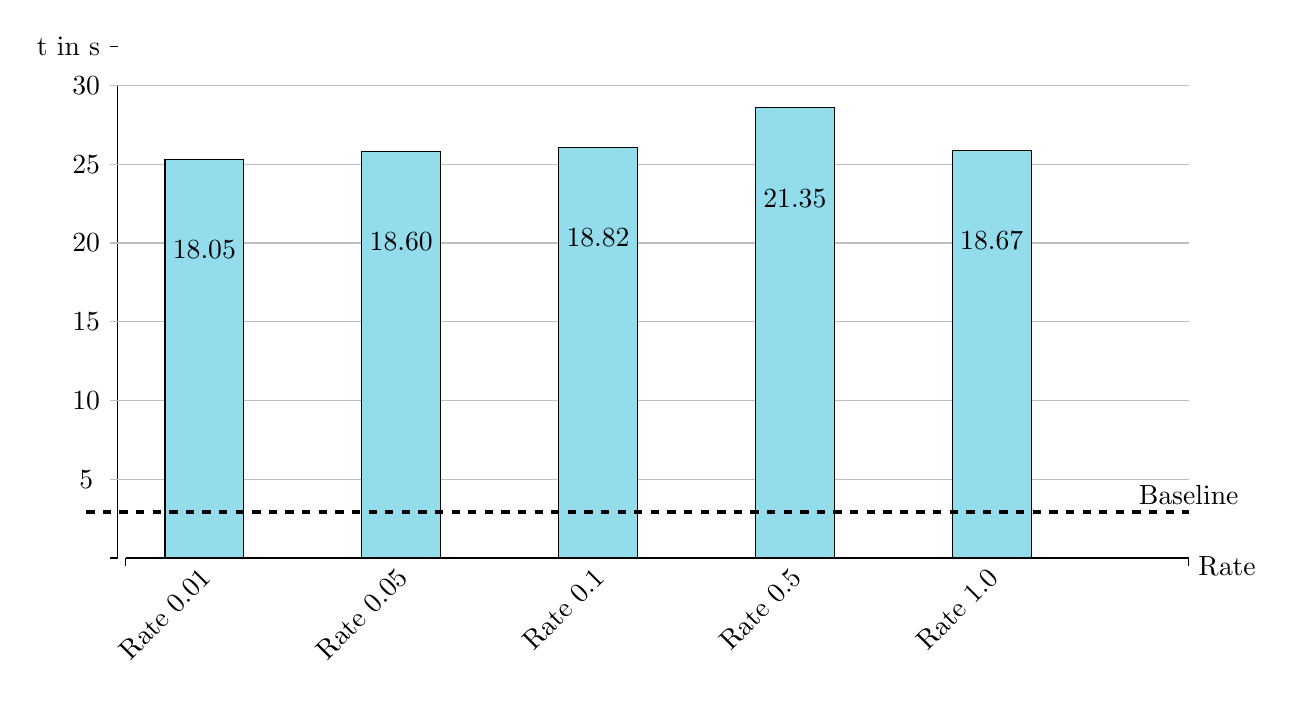
\begin{tikzpicture}
 
  \draw (0cm,0cm) -- (13.5cm,0cm);  %Abzisse
  \draw (0cm,0cm) -- (0cm,-0.1cm);  %linkes Ende der Abzisse
  \draw (13.5cm,0cm) -- (13.5cm,-0.1cm) node [right] {Rate}; %rechtes Ende der Abzisse
  
  \draw (-0.1cm,0cm) -- (-0.1cm,6cm);  %Ordinate
  \draw (-0.1cm,0cm) -- (-0.2cm,0cm);  %unteres Ende der Ordinate
  \draw (-0.1cm,6.5cm) -- (-0.2cm,6.5cm) node [left] {t in s};  %oberes Ende der Ordinate

  \foreach \x/\y in {5/1,10/2,15/3,20/4,25/5,30/6}  %Hilfslinien
    \draw[gray!50, text=black] (-0.2 cm,\y cm) -- (13.5 cm,\y cm) 
      node at (-0.5 cm,\y cm) {\x};  %Beschriftung der Hilfslinien

  %  \node at (7.5cm,7cm) {Injektionsstrategie Bitflip mit Lese- und Scheiboperationen};  %Überschrift

  \foreach \x/\y/\country in {0.5/18.05/Rate 0.01,  %\x ist Anfang der Säulen
                             % 2/2.66/Rate 0.05,  %\y ist Höhe der Säulen
                              3.0/18.60/Rate 0.05,
                             % 5/33.89/Rate 0.5,
                              5.5/18.82/Rate 0.1,
                             % 8/1.5/Niederlande,
                              8.0/21.35/Rate 0.5 ,
                             % 11/0.9/Deutschland,
                              10.5/18.67/Rate 1.0}%,
                             % 14/0.1/Italien}
    {
     \draw[fill=myblue] (\x cm,0cm) rectangle (1cm+\x cm,1.446cm + 0.2*\y cm) %die Säulen
      node at (0.5cm + \x cm,0.2*\y cm + 0.3cm) {\y}; %die Prozente über den Säulen
     \node[rotate=45, left] at (0.6 cm +\x cm,-0.1cm) {\country}; %Säulenbeschriftung
    }; 

    	\draw[black, text=black, line width=1.5pt, style=dashed] (-0.5 cm,0.2*2.892 cm) -- (13.5 cm,0.2*2.892 cm); %Baseline    
     \node at (13.5cm, 0.8cm) {Baseline};  %Überschrift  
\end{tikzpicture}

\caption[Messung Bitflip Strategie]{Injektionsstrategie Bitflip mit Lese- und Scheiboperationen}
\label{diaBitflip}
\end{figure}

\subsection*{CPU-Auslastung \& Speicherverbrauch der Strategien}

Die CPU-Auslastung und der Speicherverbrauch wurden bei einer Bl\"ockgr\"o\ss e von 1 gemessen, da diese die l\"angsten Messungen erm\"oglicht. Bei allen Strategien konnte f\"ur die CPU-Auslastung nach dem Lesen der Daten, ein konstanter Wert zwischen 12.4\% und 12.8\% ermittelt werden. Auch der Speicherverbrauch erreichte einen  konstanten Wert von ca. 440 MB. Die einzige Ausnahme im Bezug auf den Speicherbereich, bildete die Loss Strategie mit einem Wert von 490 MB. Dies ist dem Mechanismus zur Bestimmung der nicht injizierten Werte geschuldet. Es werden hierf\"ur alle Fehlerwerte in einer weiteren Datenstruktur markiert. Am Ende der Strategie findet die Daten\"ubertragung in die Ergebnisliste statt, was zusätzlich zu einem rapiden Anstieg des Speicherverbrauchs f\"uhrt. Die Messwerte diesbzgl. sind in Tabelle \ref{tblSpeicherLoss} angegeben. Es ist schnell zu erkennen das der Anstieg am Ende der Methode, abh\"angig von der Anzahl der verbliebenen Bytes ist. Bei einem Wert von 0.1 werden nur wenige Bytes entfernt, wodurch die Ergebnisliste sehr gro\ss{} ausf\"allt. Liegt die Fehlerrate allerdings bei 1.0 werden alle Bytes entfernt, wodurch die Ergebnisliste leer bleibt.

\begin{table}[!htbp]
\centering
\begin{tabular}{c|c|c|c|}
Loss & Fehlerrate & Speicher zu Beginn (MB) & Speicher bei \"Ubertragung (MB)\\
\hline
& 0.1 & 490 & 675\\
& 0.3 & 490 & 634\\
& 0.5 & 490 & 592\\
& 0.7 & 490 & 552\\
& 1.0 & 490 & 490\\
\end{tabular}
\caption{Messwerte Speicherverbrauch Loss}
\label{tblSpeicherLoss}
\end{table}



\section{Branch Prediction}\label{BranchPrediction}
Ein branch predictor in einer Computer Architekur, ist eine digitale Schaltung die versucht, den n\"achsten richtigen Weg in einer Verzweigung zu erraten, bevor dieser sicher bekannt ist. Die Tabelle \ref{tblmisprediction} zeigt exemplarisch die Zero Strategie mit den gemessenen Fehlerwerten von 0.1 bis 1.0, die Anzahl der ausgef\"uhrten Injektionen und die jeweilige Laufzeit. Man sieht beispielsweise bei einer Fehlerrate von 0.3, eine deutlich geringere Anzahl an Injektionen, als bei einer Fehlerrate von 1.0. Dennoch ist die  Laufzeit bei einer Fehlerrate von 0.3 h\"oher. Genauer l\"asst sich feststellen das Fehlerwerte die n\"aher bei 0.5 liegen, mit hoher Wahrscheinlichkeit mispredictions also Fehlvorhersagen erzeugen (ungef\"ahr eine pro Durchlauf), die Performance Einbu\ss e nach sich ziehen. Liegt der Wert hingegen nahe bei 0 oder 1 sind die branch predictions oft exakt, was die Performance erheblich beschleunigt \footnote{bei 0 oder 1 keine mispredictions}. Besonders gut wird dieses Verhalten im folgenden Diagramm ''Durschnittliche Laufzeit Zero'' verdeutlicht.  \\

\begin{table}[!htb]

\centering
\begin{tabular}{ccrr}
\hline
Zero & Fehlerrate & Anzahl Injektionen & Laufzeit in ms\\
\hline
& 0.1 & 5121757	& 2870 \\
& 0.2 & 10238034	& 3079 \\
& 0.3 & 15357873	& 3150 \\
& 0.4 & 20483144	& 3279 \\
& 0.5 & 25598114	& 3372 \\
& 0.6 & 30722540	& 3332 \\
& 0.7 & 35841016	& 3267 \\
& 0.8 & 40959774	& 3207 \\
& 0.9 & 46079605	& 3183 \\
& 1.0 & 51200000	& 3070 \\
\hline
\end{tabular}
\caption{Messwerte bzgl. Branch Prediction}
\label{tblmisprediction}
\end{table}

\begin{figure}[!htb]
\psset{xunit=0.1cm, yunit=0.1cm } 
\begin{pspicture}(-20 , -12.5)(50,72)
\psaxes[Dx=0.1, dx=10, Dy=100, dy=10, Ox=0.0, Oy=2800]{->}(110,70) 
\uput[-90](50,72.5){{Durschnittliche Laufzeit Zero}}
\uput[-90](50,-8){\textcolor{blue}{Rate}}
\uput[180]{90}(-15,30){\textcolor{blue}{Laufzeit in ms}}
\readdata{\data}{misprediction.dat} 
\listplot[showpoints=true,linecolor=red, linewidth=1.5pt]{\data}
\end{pspicture} 
\label{diaBranch}
\caption{Messung Branch Prediction}
\end{figure}

\section{Zusammenfassung}
Die ausgef\"uhrten Tests haben gezeigt, dass die Modifikation der Annotationen, selbst bei einer gro\ss en Anzahl neuer Werte, die Laufzeit kaum beeintr\"achtigt. Die CPU-Auslastung stieg kurzzeitig auf 20\% bei einem minimal ansteigenden Speicherverbrauch. Bei den Fehlerinjektionen teilt sich das Feld in drei Kategorien auf. Die Zero, BitflipB und auch die etwas aufwendigere Random Strategie, zeichnen sich durch eine schnelle Laufzeit sowie einen kostanten Speicherverbrauch aus. Die Loss Strategie ist in ihrer Laufzeit unkritisch, verursacht aber einen hohen Speicherverbrauch im letzten Abschnitt ihrer Berechnung. Dies sollte bei ihrer Verwendung ber\"ucksichtigt werden. Dagegen benötigt Bitflip f\"ur die Ausf\"uhrung erheblich mehr Zeit, weshalb alternativ die Strategie BitflipB erstellt wurde. Diese Messungen zeigen, dass die Implementierung zur Evaluation großer verteilter Systeme geeignet ist. Der gemessene CPU- und Memory-Overhead ist trotz zu erwartender gro\ss er Datenmengen in einem akzeptablen Bereich. Messungen zur Energieeffizenz dieser Systeme sollten, trotz der vorgenommenen Fehlerinjektion, weiterhin aussagekräftig bleiben.